%!TEX root = ../template.tex
%%%%%%%%%%%%%%%%%%%%%%%%%%%%%%%%%%%%%%%%%%%%%%%%%%%%%%%%%%%%%%%%%%%%
%% chapter7.tex
%% NOVA thesis document file
%%
%% Chapter with lots of dummy text
%%%%%%%%%%%%%%%%%%%%%%%%%%%%%%%%%%%%%%%%%%%%%%%%%%%%%%%%%%%%%%%%%%%%

\typeout{NT FILE chapter7.tex}%

%!TEX root = ../dissertation.tex
\chapter{Risultati Sperimentali}
\label{chapt:7}

In questo capitolo, viene presentata un'analisi approfondita dei risultati sperimentali ottenuti dall'implementazione e valutazione di diversi algoritmi risolutivi per il \textit{Travelling Salesman Problem} (TSP). Gli esperimenti sono stati condotti su una vasta gamma di istanze del problema, variando in dimensione e complessità, al fine di valutare le prestazioni degli algoritmi in termini di qualità della soluzione, tempo di esecuzione e scalabilità.

\section{Metodologia Sperimentale}
\label{sec:metodologia}

\subsection{Setup Sperimentale}
Gli esperimenti sono stati eseguiti su un cluster di calcolo (DEI Blade) con nodi equipaggiati con processori ntel Xeon Gold 5118 CPU @ 2.30/3.20GHz e 128 GB di RAM. Tutti gli algoritmi sono stati implementati in Rust.

\subsection{Istanze del Problema}
È stato utilizzato un insieme diversificato di istanze del TSP, tratte principalmente dalla TSPLIB \cite{TSPLIB}. Le istanze variano da problemi di piccole dimensioni (51 città) a problemi di grande scala (fino a 5915 città). Alcune delle istanze utilizzate includono:

\begin{itemize}
	\item eil51, berlin52, st70, eil76, pr76 (problemi di piccole dimensioni)
	\item lin105, pr124, lin318, rat575 (problemi di medie dimensioni)
	\item rat783, pr1002, pcb1173, d1655, fl1577, u2319 (problemi di grandi dimensioni)
	\item rl5915 (problema di grandissima scala)
\end{itemize}

\subsection{Algoritmi Implementati}
Sono stati implementati e valutati i seguenti algoritmi:

\begin{itemize}
	\item Nearest Neighbor (NN) e NN con 2-Opt (NN2Opt)
	\item Simulated Annealing (SA) e SA con 2-Opt (SA2Opt)
	\item Genetic Algorithm (GA) e GA con 2-Opt (GA2Opt)
	\item Ant Colony System (ACS) e ACS con 2-Opt (ACS2Opt)
	\item Red-Black Ant Colony System (RBACS) e RBACS con 2-Opt (RBACS2Opt)
\end{itemize}

\subsection{Metriche di Valutazione}
Le principali metriche utilizzate per valutare le prestazioni degli algoritmi sono:

\begin{itemize}
	\item \textbf{Tempo di esecuzione}: misurato in millisecondi.
	\item \textbf{Qualità della soluzione}: lunghezza del tour trovato.
	\item \textbf{Gap percentuale}: calcolato come $(lunghezza - ottimo) / ottimo * 100\%$, dove "ottimo" è la lunghezza del tour ottimo noto per l'istanza.
\end{itemize}

\section{Analisi dei Risultati}
\label{sec:analisi}

\subsection{Prestazioni Generali}
Dall'analisi dei dati sperimentali, emergono alcune tendenze generali:

\begin{figure}
	\begin{center}
		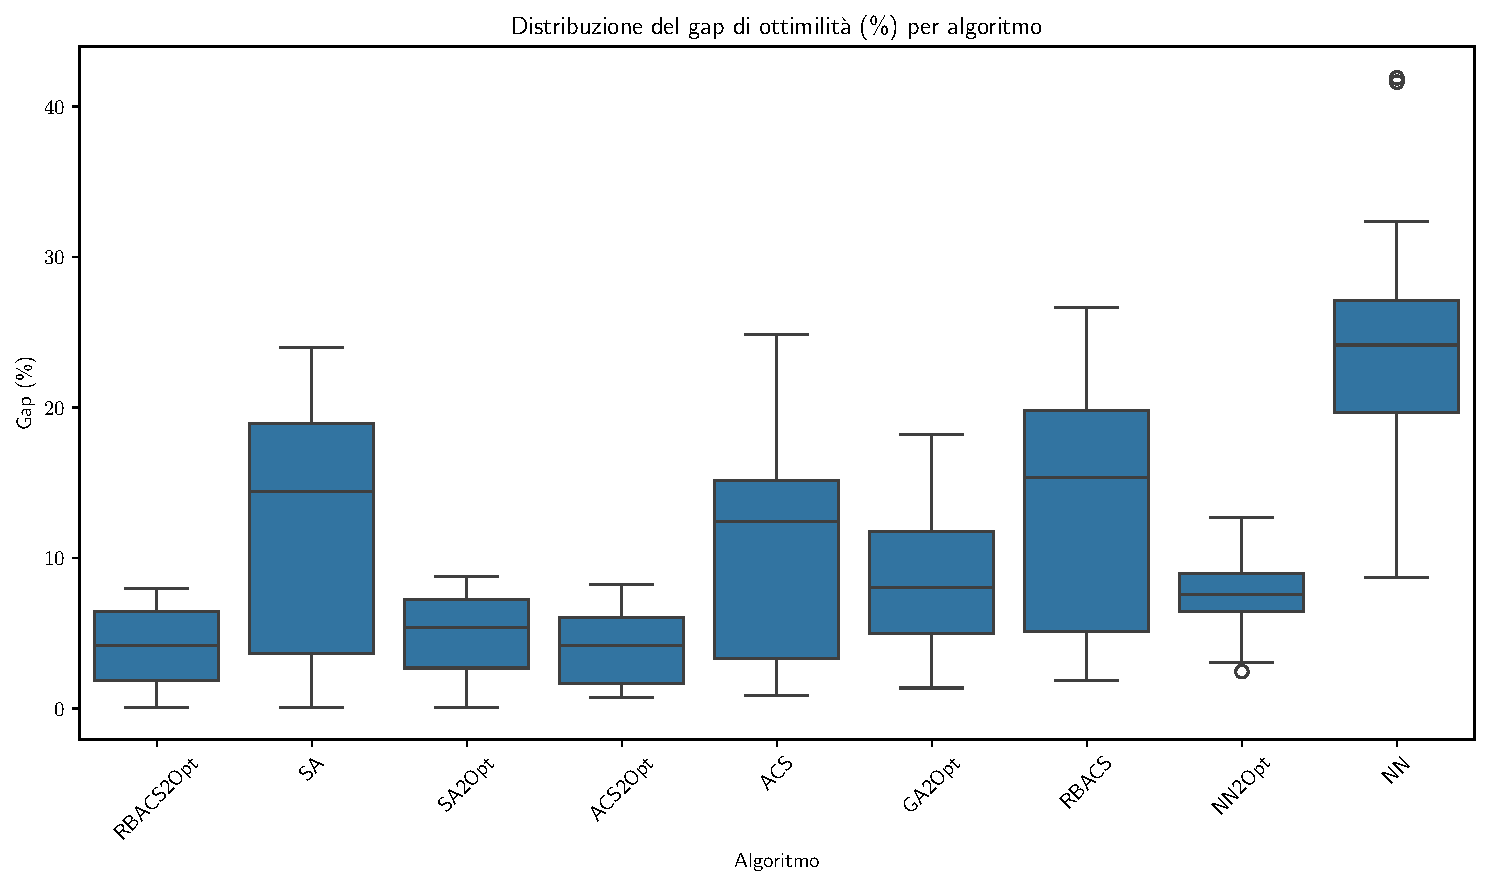
\includegraphics[width=1\textwidth]{analysis/gap_dist}
	\end{center}
	\caption{Distribuzione del gap di ottimalità per algoritmo}\label{fig:}
\end{figure}


\begin{itemize}
	\item Gli algoritmi di base (NN, SA, GA, ACS, RBACS) mostrano prestazioni significativamente migliorate quando combinati con la procedura di ottimizzazione locale 2-Opt.
	\item ACS e RBACS, insieme alle loro varianti 2-Opt, tendono a produrre soluzioni di qualità superiore rispetto agli altri approcci, specialmente per istanze di grandi dimensioni.
	\item GA mostra prestazioni altamente variabili, con alcuni risultati eccellenti ma anche alcuni estremamente scarsi, soprattutto su istanze di grandi dimensioni.
\end{itemize}

\subsection{Analisi Dettagliata per Algoritmo}


\begin{figure}
	\begin{center}
		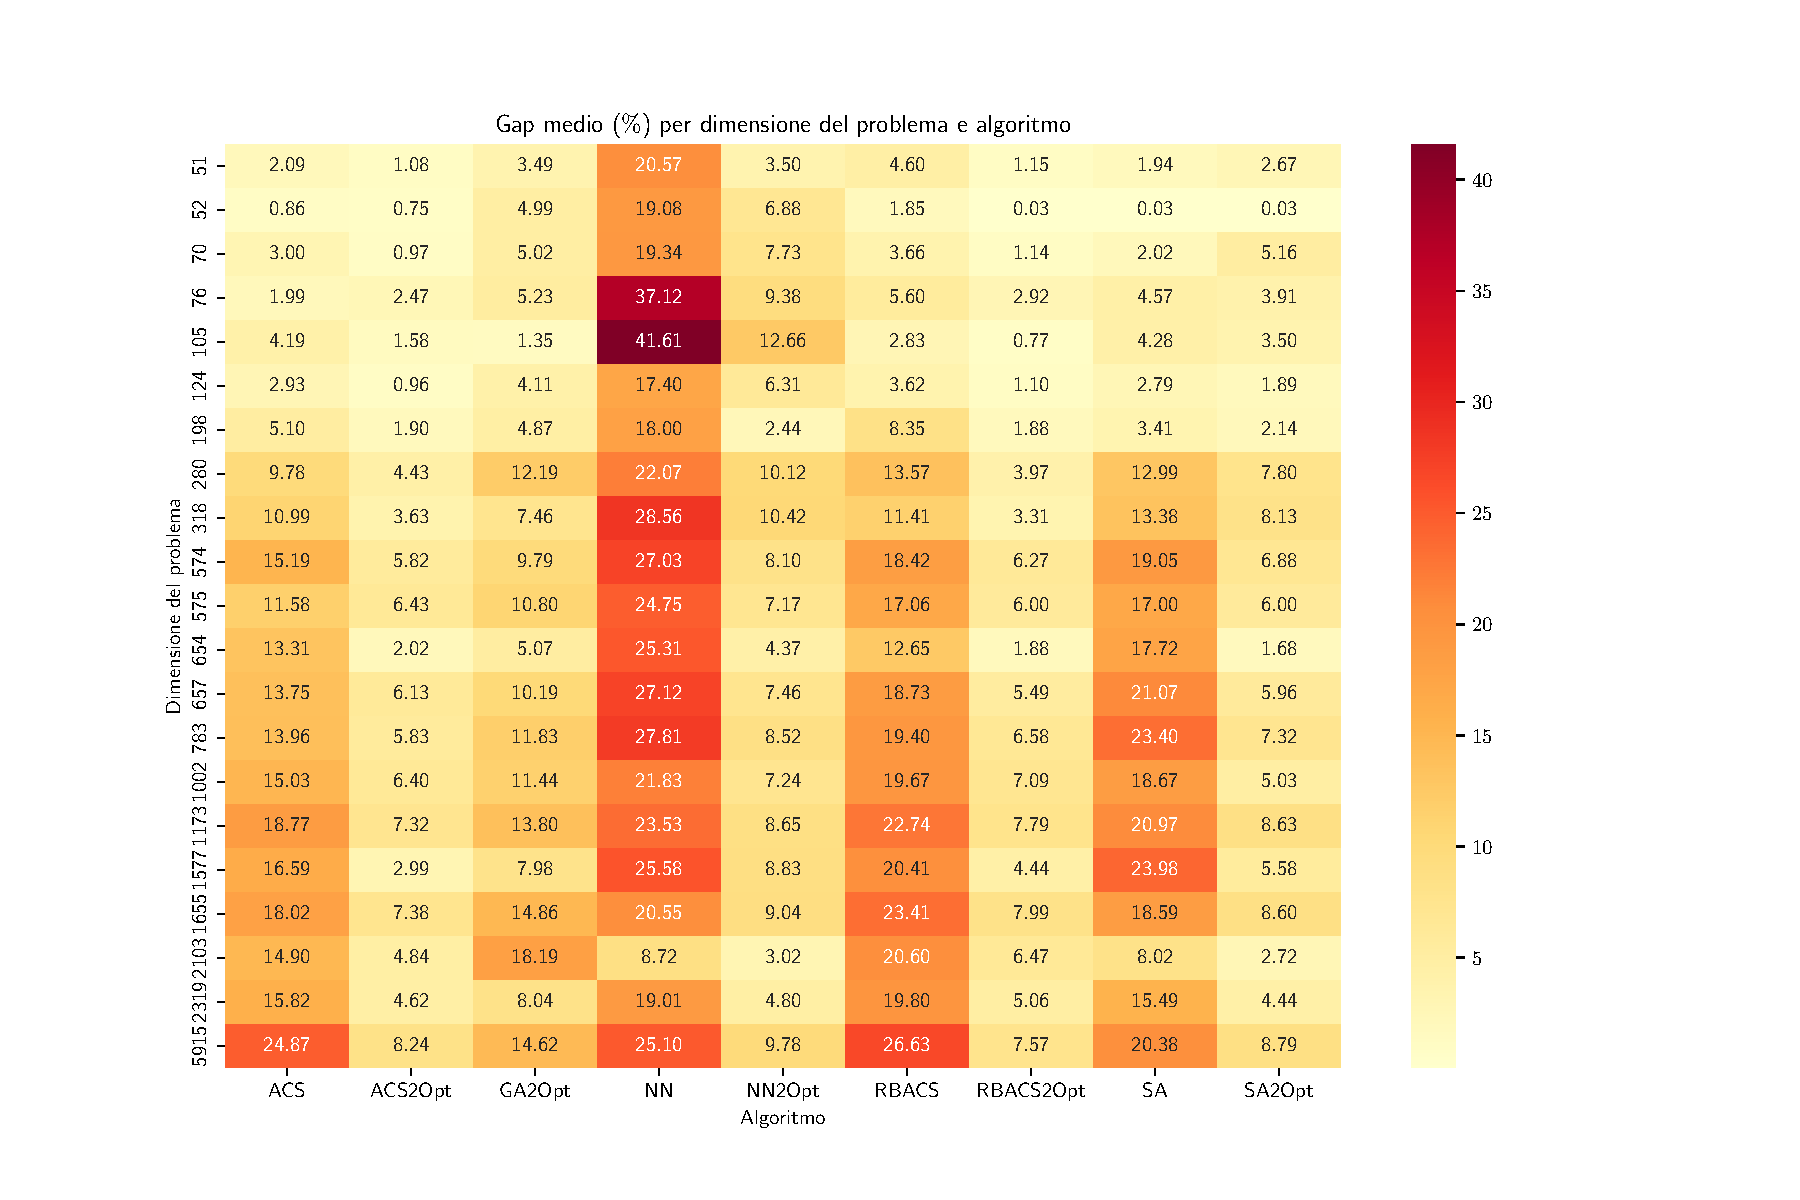
\includegraphics[width=1\textwidth]{analysis/heatmap_full}
	\end{center}
	\caption{Heatmap del gap di ottimilità}\label{fig:heatmap_full}
\end{figure}

\subsubsection{Nearest Neighbor (NN e NN2Opt)}
NN è l'algoritmo più veloce, con tempi di esecuzione che vanno da pochi millisecondi per istanze piccole a pochi secondi per istanze molto grandi. Tuttavia, la qualità delle soluzioni è generalmente inferiore rispetto agli altri approcci:

\begin{itemize}
	\item Per eil51: NN ha un gap del 20.57\%, mentre NN2Opt lo riduce al 3.50\%.
	\item Per rl5915: NN ha un gap del 25.10\%, mentre NN2Opt lo riduce al 9.78\%.
\end{itemize}

L'aggiunta di 2-Opt migliora significativamente la qualità delle soluzioni, ma aumenta il tempo di calcolo di un ordine di grandezza o più.

\subsubsection{Simulated Annealing (SA e SA2Opt)}
SA offre un buon compromesso tra qualità della soluzione e tempo di calcolo:

\begin{itemize}
	\item Per berlin52: SA raggiunge la soluzione ottima (gap 0.03\%) in 28.982 ms.
	\item Per d2103: SA2Opt ottiene un gap del 2.72\% in 7067.677 secondi.
\end{itemize}

SA2Opt generalmente produce soluzioni migliori di SA, ma con tempi di calcolo significativamente più lunghi.

\subsubsection{Genetic Algorithm (GA e GA2Opt)}
GA mostra le prestazioni più variabili tra tutti gli algoritmi testati:

\begin{itemize}
	\item Per alcune istanze piccole, come eil51, GA produce risultati scarsi (gap 41.67\%).
	\item Per istanze più grandi, come u2319, GA produce risultati estremamente scarsi (gap 2103.99\%).
	\item GA2Opt migliora significativamente le prestazioni, ma rimane meno competitivo rispetto ad ACS e RBACS per istanze di grandi dimensioni.
\end{itemize}

\subsubsection{Ant Colony System (ACS e ACS2Opt)}
ACS e ACS2Opt mostrano prestazioni molto buone su tutta la gamma di istanze:

\begin{itemize}
	\item Per berlin52: ACS ottiene un gap dello 0.86\% in 18.411 secondi, mentre ACS2Opt lo riduce allo 0.75\% in 20.289 secondi.
	\item Per fl1577: ACS2Opt ottiene un gap del 2.99\% in 3852.624 secondi.
\end{itemize}

ACS2Opt tende a produrre soluzioni di qualità leggermente superiore rispetto ad ACS, ma con tempi di calcolo più lunghi.

\subsubsection{Red-Black Ant Colony System (RBACS e RBACS2Opt)}
RBACS e RBACS2Opt mostrano prestazioni competitive e talvolta superiori rispetto ad ACS e ACS2Opt:

\begin{itemize}
	\item Per berlin52: RBACS2Opt ottiene un gap dello 0.03\% in 34.159 secondi.
	\item Per d2103: RBACS2Opt ottiene un gap del 6.47\% in 5855.328 secondi, superando ACS2Opt che ottiene un gap del 4.84\% in 4419.537 secondi.
\end{itemize}

RBACS2Opt sembra particolarmente efficace su istanze di grandi dimensioni, offrendo un buon compromesso tra qualità della soluzione e tempo di calcolo.

\subsection{Analisi della Scalabilità}
Per valutare la scalabilità degli algoritmi, è stato analizzato come il tempo di esecuzione e la qualità della soluzione variano al crescere della dimensione del problema:

\begin{figure}[h]
	\makebox[\textwidth][c]{%
		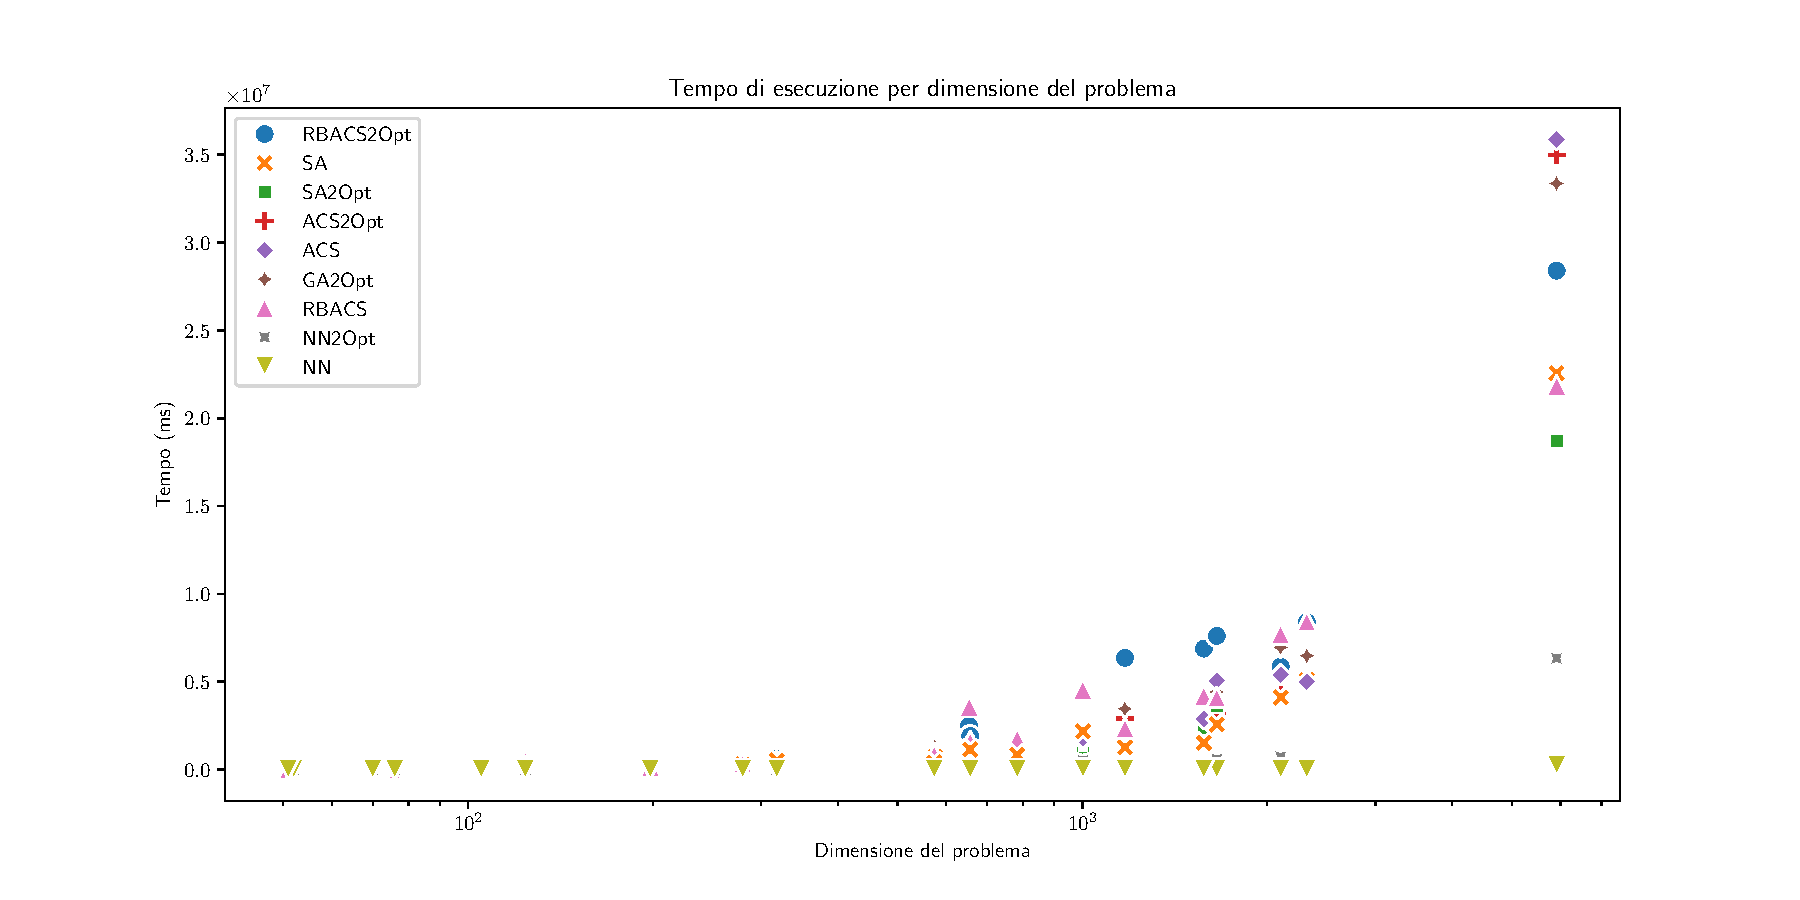
\includegraphics[width=1.2\textwidth]{analysis/time_vs_size.pdf}
	}
	\caption{Esecuzione per dimensione del problema}
	\label{fig:time_vs_size}
\end{figure}

\begin{itemize}
	\item NN e NN2Opt mostrano la migliore scalabilità in termini di tempo di esecuzione, ma la qualità della soluzione degrada rapidamente per istanze più grandi.
	\item SA e SA2Opt mantengono una buona qualità della soluzione anche per istanze grandi, ma il tempo di calcolo cresce rapidamente.
	\item GA e GA2Opt mostrano una scalabilità scarsa sia in termini di tempo che di qualità della soluzione per istanze molto grandi.
	\item ACS, ACS2Opt, RBACS e RBACS2Opt offrono il miglior compromesso tra scalabilità del tempo di esecuzione e mantenimento della qualità della soluzione per istanze di grandi dimensioni.
\end{itemize}

\begin{figure}[h]
	\makebox[\textwidth][c]{%
		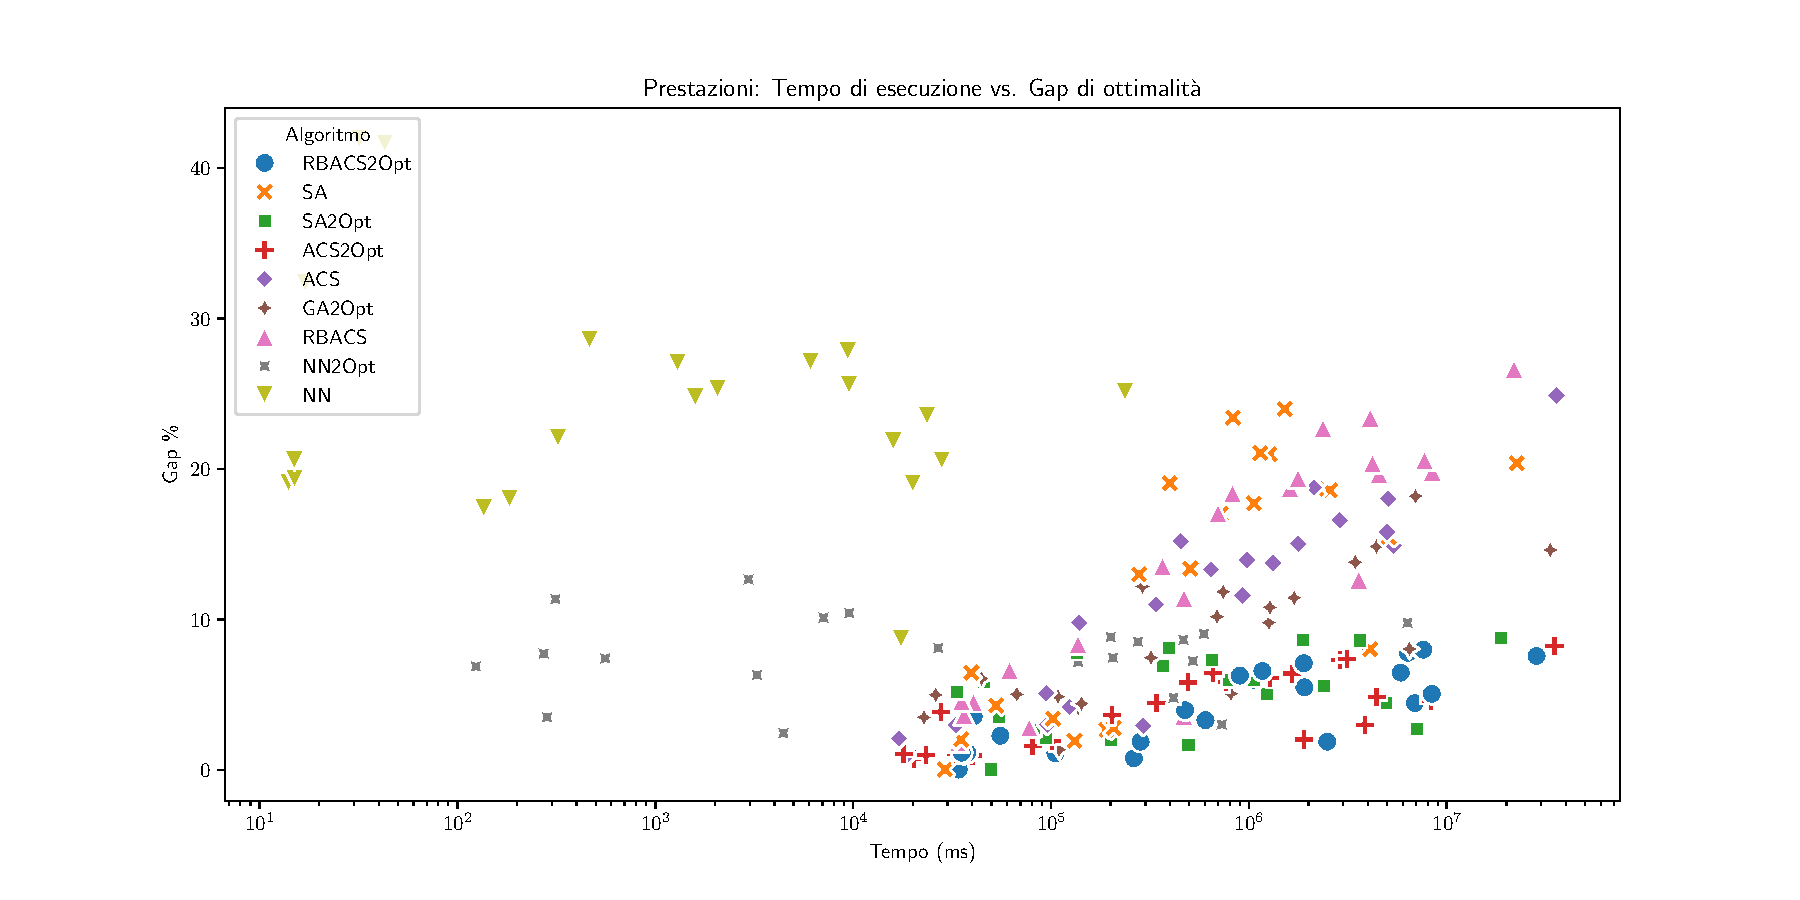
\includegraphics[width=1.2\textwidth]{analysis/time_vs_gap.pdf}
	}
	\caption{Gap per dimensione del problema}
	\label{fig:time_vs_gap}
\end{figure}

\section{Discussione}
\label{sec:discussione}

I risultati sperimentali evidenziano diversi punti chiave:

\begin{enumerate}
	\item L'importanza dell'ottimizzazione locale: l'aggiunta di 2-Opt migliora consistentemente le prestazioni di tutti gli algoritmi testati.
	\item La superiorità degli approcci basati su colonie di formiche (ACS e RBACS) per istanze di medie e grandi dimensioni.
	\item La variabilità delle prestazioni dell'algoritmo genetico, che suggerisce la necessità di un'attenta calibrazione dei parametri per ottenere buoni risultati.
	\item Il compromesso tra tempo di calcolo e qualità della soluzione, con algoritmi più sofisticati che richiedono più tempo ma producono soluzioni migliori.
\end{enumerate}

\begin{figure}[h]
	\makebox[\textwidth][c]{%
		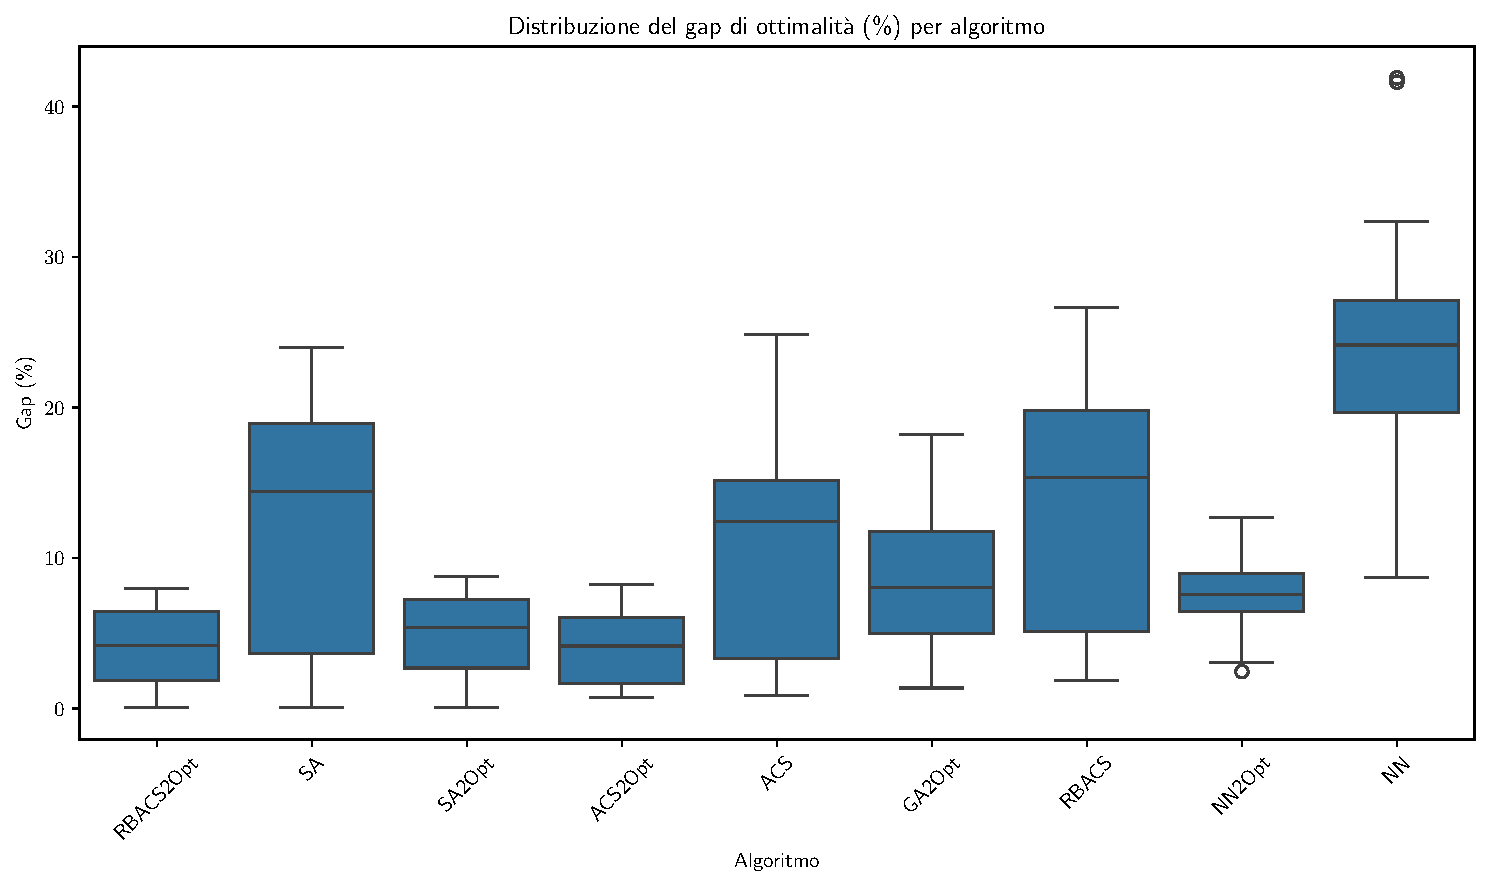
\includegraphics[width=0.75\textwidth]{analysis/alg_comparison.pdf}
	}
	\caption{Confronto tra top 3 algoritmi: Gap}
	\label{fig:alg_comparison_gap}
\end{figure}

RBACS e RBACS2Opt emergono come approcci promettenti, offrendo prestazioni competitive e talvolta superiori rispetto ad ACS e ACS2Opt, specialmente su istanze di grandi dimensioni. Tuttavia, la scelta dell'algoritmo ottimale dipende dalle specifiche esigenze dell'applicazione, bilanciando la necessità di soluzioni di alta qualità con i vincoli di tempo di calcolo.

\begin{figure}[h]
	\makebox[\textwidth][c]{%
		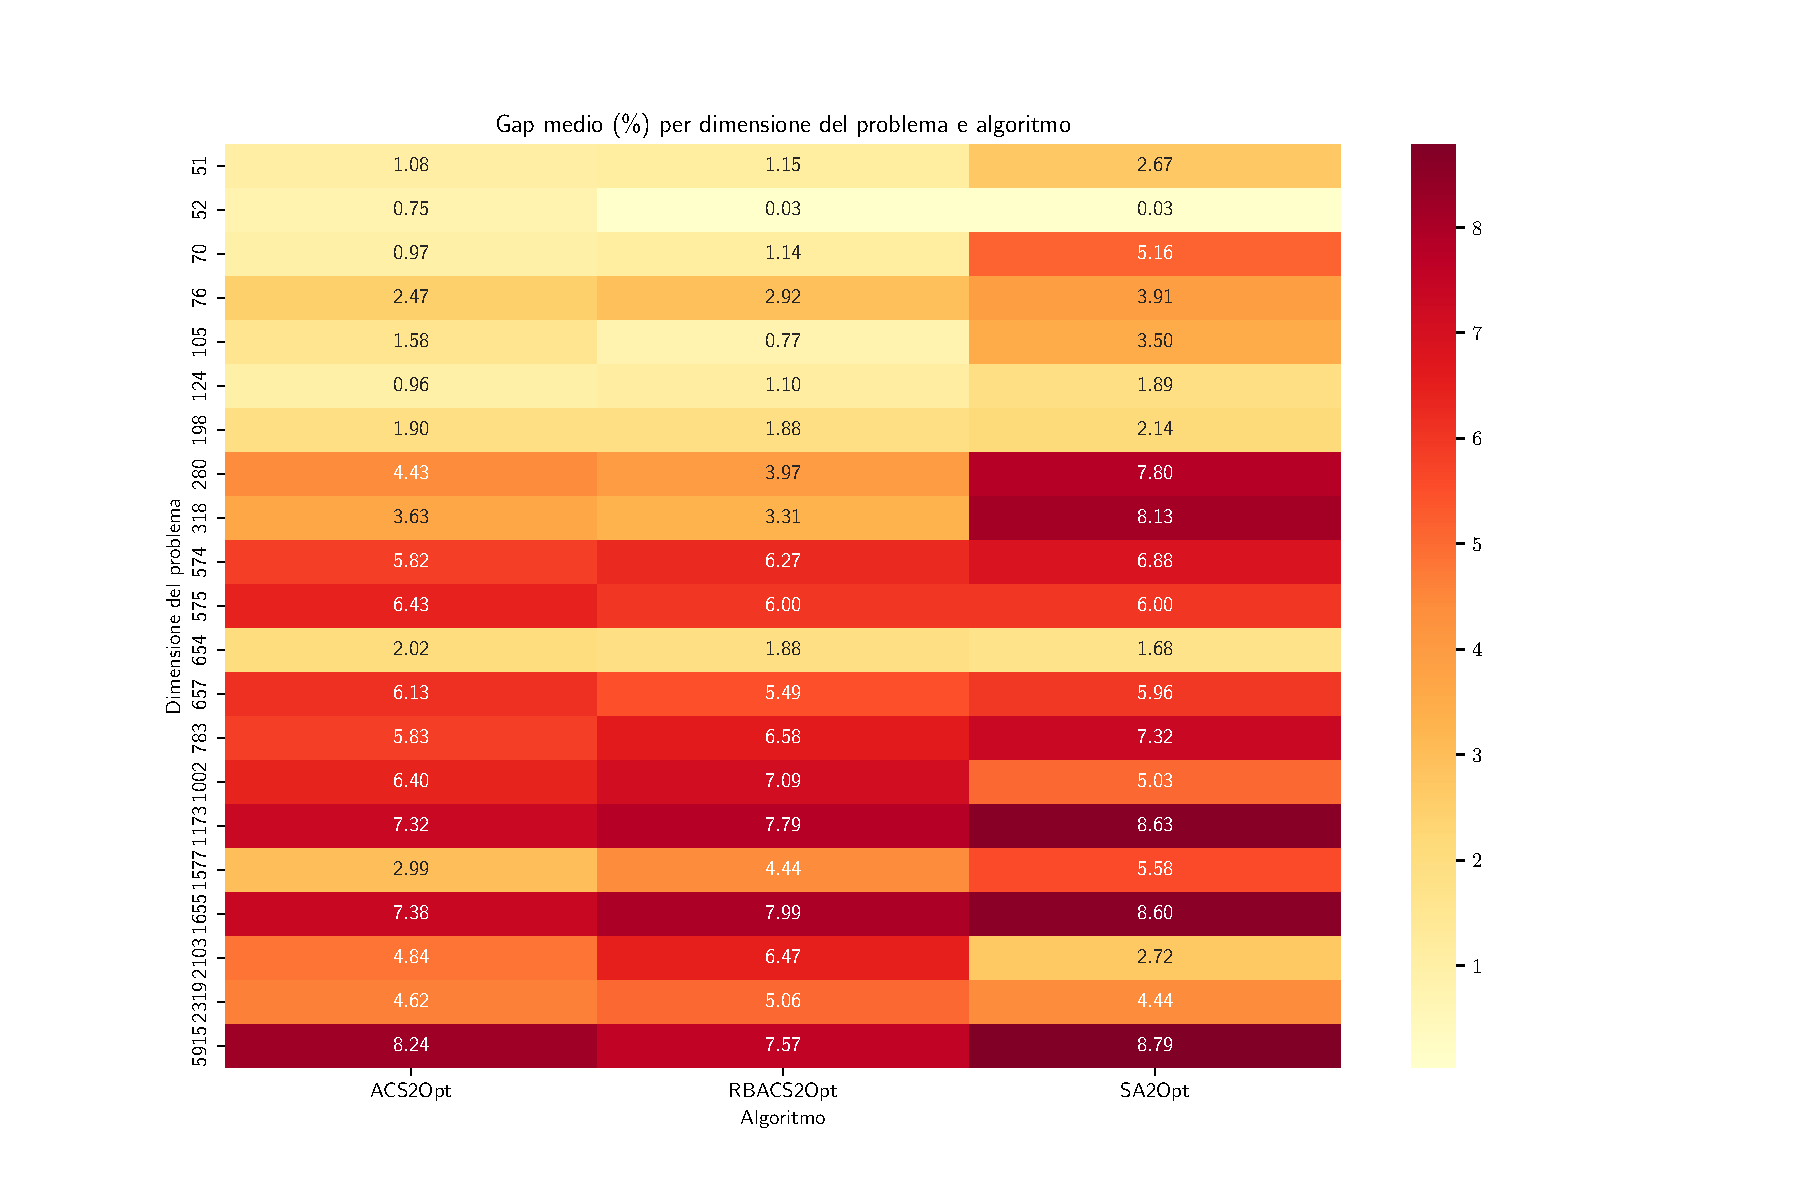
\includegraphics[width=1\textwidth]{analysis/heatmap.pdf}
	}
	\caption{Confronto tra top 3 algoritmi}
	\label{fig:alg_comparison_heatmap}
\end{figure}


\chapter{Conclusioni}
\label{chapt:8}
In conclusione, questa tesi ha fornito un'analisi approfondita e comparativa di diversi approcci algoritmici per la risoluzione del Problema del Commesso Viaggiatore, con particolare attenzione alle prestazioni su istanze di grandi dimensioni. I risultati ottenuti non solo confermano l'efficacia di approcci metaeuristici consolidati come l'Ant Colony System, ma introducono anche un nuovo algoritmo promettente, il Red-Black Ant Colony System, che mostra potenziale per ulteriori miglioramenti e applicazioni.

\section{Riflessioni Finali}
L'evoluzione degli algoritmi per il TSP riflette una tendenza più ampia nel campo dell'ottimizzazione combinatoria: la ricerca di un equilibrio tra la qualità della soluzione e l'efficienza computazionale. Questa tesi ha dimostrato che:

\begin{itemize}
	\item Non esiste un "algoritmo migliore" universale per il TSP. La scelta dell'approccio ottimale dipende dalle caratteristiche specifiche del problema, dalle dimensioni dell'istanza e dai vincoli computazionali.

	\item L'ibridazione di tecniche, come l'integrazione di procedure di ricerca locale (2-Opt) in metaeuristiche basate su popolazione, può portare a miglioramenti significativi nelle prestazioni.

	\item La scalabilità rimane una sfida cruciale, specialmente per problemi di grandissima scala (oltre 10,000 città). In questo contesto, approcci come RBACS che offrono maggiori opportunità di parallelizzazione diventano particolarmente rilevanti.

	\item La robustezza degli algoritmi, ovvero la loro capacità di mantenere buone prestazioni su una vasta gamma di istanze diverse, è un fattore critico per le applicazioni pratiche.
\end{itemize}

\section{Osservazioni Conclusive}
Il Problema del Commesso Viaggiatore, nonostante la sua apparente semplicità, continua a sfidare ricercatori e professionisti, spingendo i confini dell'ottimizzazione combinatoria e dell'informatica teorica.
